\chapter{Sensor design}

\section{Available solutions}
At the moment of writing there are few available commercial solutions. They are used in medical dosimetry, but also on spacecrafts. 

Most of commercial solutions are based on modified MOS structure (with thicker gate region). Example silicon structure is show in figure \ref{Tyndall_radfet_silicon}. Different companies produce their own RadFET devices, by designing different structure, fitted to particular requirements. Found companies produce RadFET sensor alone, leaving readout circuit design for customer. Physical phenomena for RadFET sensors is described in section \ref{Physical_phenomena_background}.

\begin{figure}[H]
	\centering
	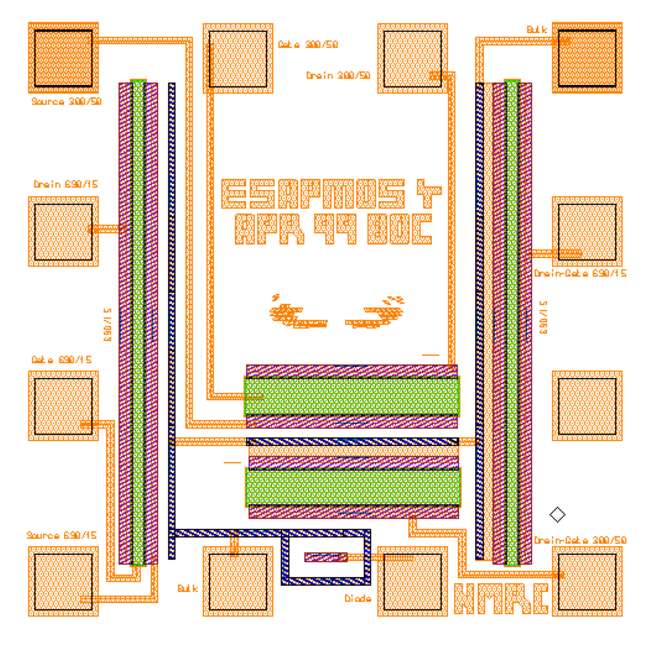
\includegraphics[width=0.5\paperwidth]{img/radfet-silicon.eps}
	\caption{4x RadFET silicon structure by Tyndall. Source: \cite{Tyndall_Radfet}}
	\label{Tyndall_radfet_silicon}
\end{figure}


Available products on market:

\subsection{REM Oxford}
	REM Oxford \cite{RADFET_COM_URL}. This company produces RadFET type RFT300-CC10G1, its datasheet can be found on \cite{RFT300_CC10G1}. Structure is mounted on small carrier, as shown on figure \ref{REM_radfet_drawing}.
	
	\begin{figure}[H]
		\centering
		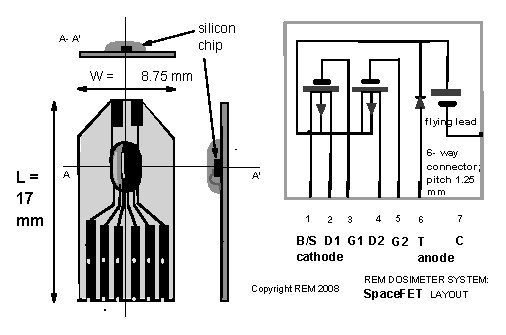
\includegraphics[width=0.5\paperwidth]{img/remOxfordDrawing.eps}
		\caption{RadFET made by REM Oxford. Source: \cite{RFT300_CC10G1}}
		\label{REM_radfet_drawing}
	\end{figure}
	
	This sensor consists of two PMOS transistors with modified gate structure.
	
	Key features:
	\begin{itemize}
		\item gate thickness \SI{200}{\nano\meter}, \SI{250}{\nano\meter} or \SI{300}{\nano\meter},
		\item sensitivity $\SI{1.5}{\milli\volt/\centi\gray} = \SI{1.5}{\milli\volt/\rad}$. Sensitivity chart is shown on figure \ref{REM_radfet_sensitivity}. At required sensitivity (\SI{1}{kRad}) threshold voltage shifts by $>\SI{100}{\milli\volt}$, depending on configuration,
		\item fading of shift is shown on figure \ref{REM_radfet_fading} - it is negligible on required mission duration ($<~\SI{3}{\percent}$),
		\item manufacturer suggests readout current in range $10-\SI{500}{\micro\ampere}$,
		\item sensor includes temperature readout from on-die diode
	\end{itemize}

	Price for one RadFET sensor begins from 800~\$.
	
	\begin{figure}[H]
		\centering
		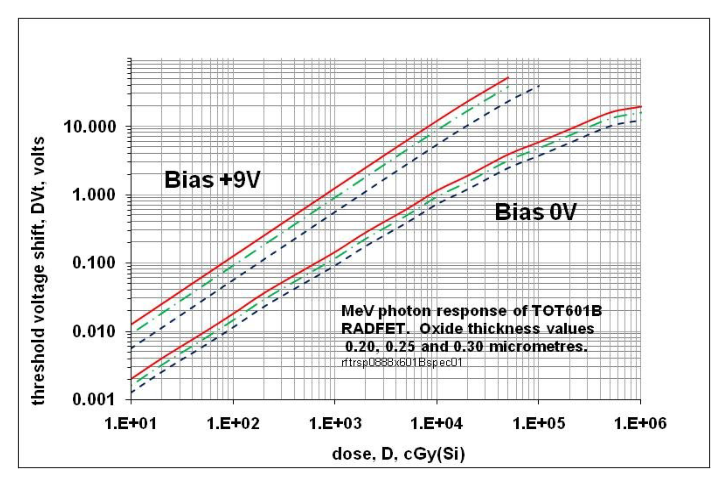
\includegraphics[width=0.6\paperwidth]{img/remSensitivity.eps}
		\caption{REM Oxford RadFET sensitivity. Source: \cite{RFT300_CC10G1}}
		\label{REM_radfet_sensitivity}
	\end{figure}
	
	\begin{figure}[H]
		\centering
		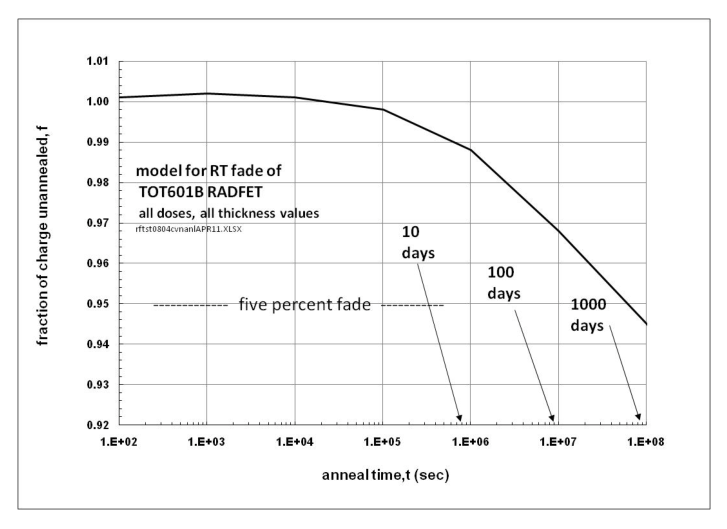
\includegraphics[width=0.6\paperwidth]{img/remOxfordFading.eps}
		\caption{REM Oxford RadFET fading. Source: \cite{RFT300_CC10G1}}
		\label{REM_radfet_fading}
	\end{figure}


\subsection{Tyndall}
	Tyndall Works manufactures RadFET components in different packaging options \cite{TYNDALL_URL}. They provide calibration data for each type of sensor, as their response is very non-linear. Graph showing sensitivity of TY1002 is shown on figure \ref{Tyndall_TY1002_sensitivity}. Tyndall provide 4 different options, their comparison is done in table \ref{Tyndall_comparison}. Tyndall recommends grounding RadFET terminals during irradiation.
	
	\begin{figure}[H]
		\centering
		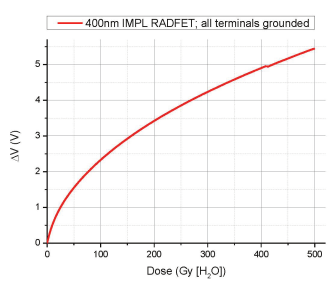
\includegraphics[width=0.6\paperwidth]{img/Tyndall_TY1002_sensitivity.png}
		\caption{Tyndall TY1002 sensitivity. Source: \cite{TYNDALL_URL}}
		\label{Tyndall_TY1002_sensitivity}
	\end{figure}
	
	\begin{table}[H]
	\begin{tabular}{| L{3.5cm} | C{2.5cm} | C{2.5cm} | C{2.5cm} | C{2.5cm} |}
		\hline
		Type: & TY1001 & TY1002 & TY1003 & TY1004 \\ \hline
		
		Image: &
		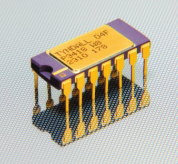
\includegraphics[width=0.12\paperwidth]{img/TY1001.png} & 
		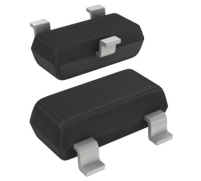
\includegraphics[width=0.12\paperwidth]{img/TY1002.png} & 
		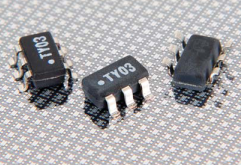
\includegraphics[width=0.12\paperwidth]{img/TY1003.png} & 
		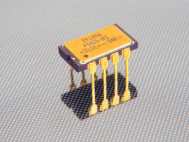
\includegraphics[width=0.12\paperwidth]{img/TY1004.png} \\ \hline

		Package: & 14-pin ceramic DILpin ceramic DIpin ceramic DI & SOT-23 & SOT23-6 & 8-pin ceramic DIL \\ \hline
		
		\# of transistors: & 4 & 1 & 2 & 2 \\  \hline
		W/L : & 300/50 \& 690/15 & \multicolumn{3}{c|}{300/50}  \\  \hline
		Oxide thickness: & - & - & \multicolumn{2}{c|}{\SI{400}{\nano\meter}} \\  \hline

		Maximum dose: & \multicolumn{4}{c|}{\SI{100}{\kilo\rad}} \\  \hline
		Minimal detectable dose: & \multicolumn{4}{c|}{\SI{1}{\rad}} \\  \hline 
				
		Recommended readout current: & \multicolumn{2}{c|}{\SI{12.5}{\micro\ampere}} & \multicolumn{2}{c|}{\SI{10}{\micro\ampere}} \\ \hline
		
		Temperature readout: & diode & none & diode & diode \\ \hline
	\end{tabular}
	\caption{Tyndall RadFET comparison}
	\label{Tyndall_comparison}
	\end{table}



\section{Proposed TID measurement technique}
\subsection{Physical phenomena background}
\label{Physical_phenomena_background}

\section{Die temperature measurement}
As the threshold voltage temperature 
\subsection{Build-in ESD diode}
\subsection{Body diode}
\section{Bias of MOSFET gate}

\section{Idea block diagram}

\section{Components selection}
\subsection{MOSFET}
\subsection{ADC}
\subsection{Microcontroller}
\subsection{Passives}

\section{Tradeoff analysis}
During sensor design tradeoff analysis was performed to tailor sensor requirements to constrains applicable (space, power, available integrated circuits). That leaded to final block diagram which sums up all information gathered during design phase.

\subsection{Measurement channels}
\subsection{Measurement accuracy}


\section{Final block diagram}